\section{Scattering by system \cite{Astafiev2010}}
\begin{framed}\noindent
  \textbf{Main result:}
  \begin{equation}\label{key}
    2ikV_{sc} = i\omega \phi_p\iaverage{\sigma_{-}}.
  \end{equation}
\end{framed}

\begin{figure}[h]
  \centering 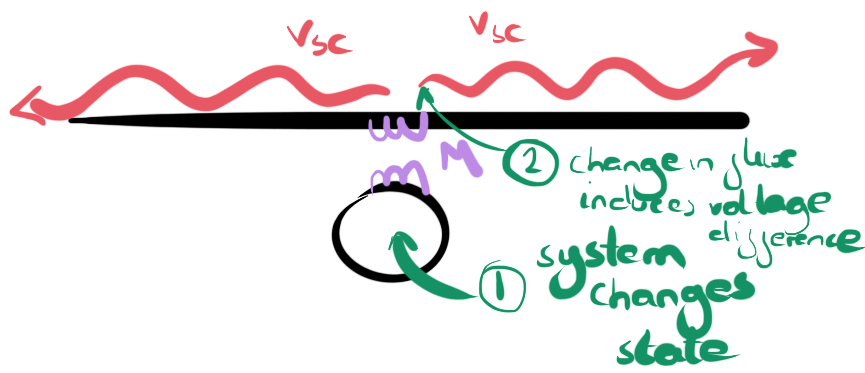
\includegraphics[height=5cm]{scattering}
\end{figure}

\noindent

\begin{enumerate}
\item  Beggining   with  the  telegraph  equations   for  the  voltage
  difference at the position of the atom:
  \begin{equation}\label{7thFeb1}
    \left\lbrace\begin{aligned}
        \frac{d\Delta V}{dx} & = l\frac{dI}{dt}\\
        \Delta V & = \iabs{V_{sc}}\left[e^{i(kx - \omega t)} - e^{i(-kx - \omega t)}\right]
      \end{aligned}\right. \Rightarrow \frac{d\Delta V}{dx} = 2ikV_{sc}
  \end{equation}

\item Now, the atom is situated specific point on the line, $ x = 0 $,
  \red{\textbf{and only  at this point is  the voltage discontinous.}}
  Thus we incoporate delta function into Eq.~\eqref{7thFeb1}
  \begin{equation}\label{7thFeb4}
    \frac{d\Delta V}{dx} = 2ikV_{sc}\delta(x)
  \end{equation}

\item This voltage  is caused by a change of  the linked flux (dipole)
  during a transition (Eq.~\eqref{dipole_2level})

  \begin{equation}\label{key}
    \text{small change in flux } = \vartheta_{ij}(t) = MI_p\isigmaminus e^{i\omega t}.
  \end{equation}

\item Let's evaluated the induced voltage due to this changing of flux

  \begin{equation}\label{7thFeb5}
    \Delta V = \dot{\Phi} = i\omega MI_p\isigmaminus e^{i\omega t}
  \end{equation}

\item     Integrating    Eq.~\eqref{7thFeb4}     and    subbing     in
  Eq.~\eqref{7thFeb5} we arrive at

  \begin{equation}\label{7thFev5}
    2ikV_{sc} = i\omega\phi_p\iaverage{\sigma_{-}}\qquad \phi_p = MI_pe^{i\omega t}
  \end{equation}

\end{enumerate}

\subsection{Coherent  dynamics and  decoherence  in a  superconducting
  weak link \cite{Peltonen_2016}}
\label{sec:coher-dynam-decoh}

Here  authors say  that dissipation  is caused  by resistance  $R_{q}$
parallel to the inductance:

\begin{equation}
  S_{i}(\omega_{q}) = \frac{2\hbar\omega_q}{2\pi R_q}
\end{equation}

\noindent which causes a relaxation rate

\begin{equation}
  \Gamma_1 = \frac{2\pi S_i(\omega_q) \varphi_p^2\sin^2\left( \theta \right)}{\hbar^2}
\end{equation}

\noindent                          where                          from
$\Delta    E    =     \sqrt{(2I_p\delta\Phi)^2+E_s^2},    \tan(\theta)    =
\frac{E_s}{2I_p\delta\Phi}$ (see \autoref{sec:qps}) we define $\theta$
and $\varphi_p = L_{q}I_p = \frac{1}{2}\Phi_0$ is the dipole moment of
the loop coupled to the resistance (not clear at all).


%%% Local Variables:
%%% mode: latex
%%% TeX-master: "all_the_notes"
%%% End:
